

\tikzset{every picture/.style={line width=0.75pt}} %set default line width to 0.75pt        

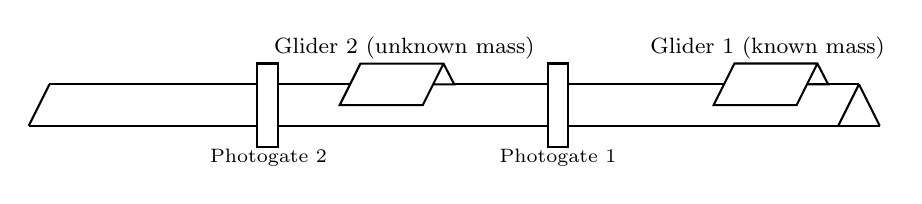
\begin{tikzpicture}[x=0.75pt,y=0.75pt,yscale=-1,xscale=1]
%uncomment if require: \path (0,300); %set diagram left start at 0, and has height of 300

%Straight Lines [id:da5572434639926174] 
\draw    (110,140) -- (520,140) ;


%Straight Lines [id:da02244511382700587] 
\draw    (110,140) -- (120,120) ;


%Straight Lines [id:da5497476983892675] 
\draw    (120,120) -- (510,120) ;


%Straight Lines [id:da57322939128216] 
\draw    (510,120) -- (520,140) ;


%Straight Lines [id:da2970462263374636] 
\draw    (510,120) -- (500,140) ;


%Shape: Rectangle [id:dp04813805212125999] 
\draw  [fill={rgb, 255:red, 255; green, 255; blue, 255 }  ,fill opacity=1 ] (220,110) -- (230,110) -- (230,150) -- (220,150) -- cycle ;
%Shape: Rectangle [id:dp8954323751602662] 
\draw  [fill={rgb, 255:red, 255; green, 255; blue, 255 }  ,fill opacity=1 ] (360,110) -- (370,110) -- (370,150) -- (360,150) -- cycle ;
%Shape: Polygon [id:ds012853840364027702] 
\draw  [fill={rgb, 255:red, 255; green, 255; blue, 255 }  ,fill opacity=1 ] (450,110) -- (490,110) -- (495.15,119.98) -- (485,120) -- (490,110) -- (480,130) -- (440,130) -- cycle ;
%Shape: Polygon [id:ds6910058608548333] 
\draw  [fill={rgb, 255:red, 255; green, 255; blue, 255 }  ,fill opacity=1 ] (269.85,110.02) -- (309.85,110.02) -- (315,120) -- (304.85,120.02) -- (309.85,110.02) -- (299.85,130.02) -- (259.85,130.02) -- cycle ;

% Text Node
\draw (365,155.5) node  [font=\footnotesize] [align=left] {{\scriptsize Photogate 1}};
% Text Node
\draw (225.5,155.5) node  [font=\footnotesize] [align=left] {{\scriptsize Photogate 2}};
% Text Node
\draw (291,102.5) node  [font=\scriptsize] [align=left] {{\footnotesize Glider 2 (unknown mass)}};
% Text Node
\draw (466,102.5) node  [font=\scriptsize] [align=left] {{\footnotesize Glider 1 (known mass)}};


\end{tikzpicture}
